\documentclass[10pt,a4jpaper]{jsarticle}
\usepackage[dvipdfmx]{graphicx}
\usepackage[dvipdfmx]{color}
\usepackage{listings}
% to use japanese correctly, install jlistings.
\lstset{
  basicstyle={\small\ttfamily},
  identifierstyle={\small},
  commentstyle={\small\itshape\color{red}},
  keywordstyle={\small\bfseries\color{cyan}},
  ndkeywordstyle={\small},
  stringstyle={\small\color{blue}},
  frame={tb},
  breaklines=true,
  numbers=left,
  numberstyle={\scriptsize},
  stepnumber=1,
  numbersep=1zw,
  xrightmargin=0zw,
  xleftmargin=3zw,
  lineskip=-0.5ex
}
\lstdefinestyle{customCsh}{
  language={csh},
  numbers=none,
}
\lstdefinestyle{customRuby}{
  language={ruby},
  numbers=left,
}
\lstdefinestyle{customTex}{
  language={tex},
  numbers=none,
}
\lstdefinestyle{customJava}{
  language={java},
  numbers=left,
}
\begin{document}
\title{hiki2latex}
\author{関西学院大学・理工学部・西谷滋人}
\date{\today}
\maketitle

\abstract{
hiki formatで書かれた文章を,latex formatに変換する

}
\tableofcontents
\section{【documents】}\begin{itemize}
\item \verb|http://rubygems.org/gems/hiki2latex|
\end{itemize}
\section{【使用法】}\begin{lstlisting}[style=customCsh]
Usage: hiki2latex [options] FILE
    -v, --version                    show program Version.
    -l, --level VALUE                set Level for output section.
    -p, --plain FILE                 make Plain document.
    -b, --bare FILE                  make Bare document.
        --head FILE                  put headers of maketitle file.
        --pre FILE                   put preamble file.
        --post FILE                  put post file.
        --listings                   use listings.sty for preformat with style.
\end{lstlisting}\begin{itemize}
\item より詳細な使用法は,\verb|hiki2latex_gemizing|にある.
\item 西谷研の内部で利用するときに特化したマニュアルは\verb|こちら(hiki2latex_manual)|.
\end{itemize}
\subsection{sample}
幾つかのサンプルを以下に示す.

\begin{table}[htbp]\begin{center}
\caption{hiki2latexにより作成されたpdfファイトとその元ネタ.}
\begin{tabular}{lll}
\hline
ソース(hiki表示)  &pdf(latex変換後)  \\ \hline
\verb|Shunkuntype(https://github.com/daddygongon/shunkuntype/wiki/Shunkuntype_report)|  &\verb|Shunkuntypeのレポート(https://github.com/daddygongon/shunkuntype/wiki/shunkun_report.pdf)|  \\
\verb|LPSO15研究会の例(LPSO15_fall_meeting_abst)|  &\verb|{{attach_anchor(LPSO_abst.pdf)}}|  \\
\verb|中間発表hand out例(AbstSample)|  &\verb|{{attach_anchor(AbstSample.pdf)}}|  \\
\verb|使っているformat集(DocumentFormatter_format_examples)|  \\
\hline
\end{tabular}
\label{default}
\end{center}\end{table}
%for inserting separate lines, use \hline, \cline{2-3} etc.

\section{【仕様】}\begin{enumerate}
\item hikdoc.rbにwrap
\item header部を独立して提供
\item author, titleはheadに手を加えて提供
\item 図はattach\_viewを変換
\item 表はそのまま表示\begin{enumerate}
\item tableのmulti対応
\end{enumerate}
\item captionはheaderで提供
\item citeは対応しない.
\item graph, tableは[h]で提供.
\end{enumerate}
\section{【具体的な使用例rakefile】}
具体的な使用例として\verb|Shunkuntype_report|を作成した時のRakefile.rbを示す.何度も書き直す時は,このようにして自動化すべき.
\begin{lstlisting}[style=customRuby]
task :shunkuntype do
  dir = '~/Sites/nishitani0/Internal/data/text/'
  targets =["Shunkuntype_manual","Shunkuntype_gemizing","TouchTyping_Coding"]
  targets.each{|file|
    p command= "rm -f #{file}.tex"
    system command
    p command= "hiki2latex -l 2 --listings -b #{dir}#{file} > #{file}.tex"
    system command
  }
  file="Shunkuntype_report"
  p command= "rm -f #{file}.tex"
#  p command= "hiki2latex --listings --head head.tex --post post.tex -p #{dir}#{file} > #{file}.tex"
  p command= "hiki2latex --listings --post post.tex -p #{dir}#{file} > #{file}.tex"
  system command

  p command = "open #{file}.tex"
  system command
  exit
end
\end{lstlisting}
本文(Shunkuntype\_report.tex)と付録(targets.texs)がある.付録は'-l 2 -b'によってsubsectionからのtitle levelにしてbare modeで作っている.post.texにpostで付け加えるtex部を指定して,appendixをつけている.

\section{【変更履歴,内容】}
変更履歴,内容を表に示す.15/8月期で基本開発.16/2月期にgem化.

\begin{table}[htbp]\begin{center}
\caption{変更履歴,内容}
\begin{tabular}{llll}
\hline
memo   &date  &hiki  \\ \hline
hikidoc.rbからhiki2latex.rb  &15/8/4  &\verb|hiki2latex_init|  \\
hiki2latex.rbひな形作成  &15/8/5  \\
@fをStringIOからStringへ  &15/8/5  \\
graph+caption  &15/8/6  &\verb|LPSO15_fall_meeting_abst|  \\
math  &15/8/7  &\verb|hiki2latex_math|  \\
table  &15/8/8  &\verb|hiki2latex_table|  \\
under\_score  &15/8/11   &\verb|hiki2latex_math|  \\
gem化  &16/2/13   &\verb|hiki2latex_gemizing|  \\
listings  &16/2/16   &\verb|hiki2latex_listings|  \\
\hline
\end{tabular}
\label{default}
\end{center}\end{table}
%for inserting separate lines, use \hline, \cline{2-3} etc.

\section{【開発メモ】}
\subsection{制限事項}\begin{itemize}
\item title中へuriの埋め込みが未対応.\begin{itemize}
\item uriのverbがlatexのtitle内で使えないため.
\end{itemize}
\end{itemize}
\subsection{【 保留項目】}\begin{enumerate}
\item includegraphicsの自動提供\begin{enumerate}
\item hikiに置かれているgraphは劣化版なんでそれをいじるのはあまり筋がよろしくない.
\item epsならできるかも.hikiのattach\_viewでサイズをどういじっているか...
\end{enumerate}
\item underbar(\_)がlatexでは全て引っかかる.escapeする?-> 対応済み \verb|hiki2latex_math|\begin{enumerate}
\item snake表記はrubyではfile名や変数名に頻繁に使われるので対処が必要かも.
\end{enumerate}
\end{enumerate}
\subsection{【math】}
$$での変換がうまくいかない.
\begin{quote}\begin{verbatim}
hikiconf.rb
\end{verbatim}\end{quote}
での設定を
\begin{quote}\begin{verbatim}
#@style           = 'default'
@style           = 'math'
\end{verbatim}\end{quote}
としたらhikiからエラーは出なくなったが.まだまだ....

\subsection{【user def】}\begin{quote}\begin{verbatim}
\def\Vec#1{\mbox{\boldmath $#1$}}
\end{verbatim}\end{quote}
はpreambleに置くことが推奨されているが,実際は,使用するまでに定義すればいい.preambleをいじるようになるころには,latexについての十分な経験があると思われるので,hiki2latexではいじらない.ちょこっと必要ならhiki本文中に埋め込むべし.今の仕様では,
\begin{lstlisting}[style=customRuby]
  def initialize(file_name)
    @buf = ""
    @buf << HEADER+"\n"
    @buf <<  "\\begin{document}\n"
    @buf <<  HikiDoc.to_latex(file_name)+"\n"
    @buf <<  REFERENCE+"\n"
    @buf << "\\end{document}\n"
  end

  def display
    @buf
  end
\end{lstlisting}
とするのが正しそうなので,無理に入れていない.将来はpreambleを保持するような拡張機能(option)が必要かもしれない.それは,「原典一つ主義」で,hikiを原典とするか,latexを原典とするかの選択が迫られたとき.
\begin{itemize}
\item\begin{itemize}
\item 追記(2015/02/17) いい考察だ.解はでてないが今はhiki2latexに埋め込んで,それらの仕様をできるだけ吸収しようとしている.
\end{itemize}
\end{itemize}
\appendix
\section{詳細な使用法}

\subsubsection{【概要】}
hikiフォーマットの記述をlatexフォーマットに変換する

\subsubsection{【使用法】}
gem化して配布可能とした.したがって,installがちゃんとできていれば,
\begin{description}
\item[command lineから] 

\end{description}\begin{lstlisting}[style=customCsh]
bob% hiki2latex Shunkuntype_manual > tmp.tex
\end{lstlisting}\begin{description}
\item[libraryとして] 

\end{description}\begin{lstlisting}[style=customRuby]
require 'hiki2latex'

puts HikiDoc.to_latex(File.read(ARGV[0]))
\end{lstlisting}\begin{lstlisting}[style=customCsh]
bob% ruby trans.rb ./Shunkuntype_manual > tmp.tex
\end{lstlisting}
などとして利用できる.

\subsubsection{【help】}\begin{lstlisting}[style=customCsh]
bob% hiki2latex
Usage: hiki2latex [options]
    -v, --version                    show program Version.
    -l, --level VALUE                set Level for output section.
    -p, --plain FILE                 make Plain document.
    -b, --bare FILE                  make Bare document.
        --head FILE                  put headers of maketitle file.
        --pre FILE                   put preamble file.
        --post FILE                  put post file.
\end{lstlisting}
\subsubsection{【詳細使用例(-p)】}
以下のようなSampleDoc
\begin{lstlisting}[style=]
bob% cat SampleDoc 
!title
contents
*list1
*list2
!!title2
\end{lstlisting}
を
\begin{lstlisting}[style=customTeX]
bob% hiki2latex -p SampleDoc 
\documentclass[12pt,a4paper]{jsarticle}
\usepackage[dvipdfmx]{graphicx}
\begin{document}
\section{title}
contents
\begin{itemize}
\item list1
\item list2
\end{itemize}
\subsection{title2}
\end{document}
\end{lstlisting}
となる.

\subsubsection{【詳細使用例(-b)】}
上記
\begin{lstlisting}[style=customTeX]
 \begin{document}
 ...
 \end{document}
\end{lstlisting}
の中身だけを生成.いくつものtex filesをincludeしている場合の個別ファイル作成に便利.

この際,'-l 2'として付録のsectionとかを調整する.

\subsubsection{【詳細使用例( --head,  --pre,  --post】}
formatを標準と違うものにするために,pre,head,postがある.詳しくはsampleを見よ.
していしていく順番はないはずだけど,-p SampleDocだけは順番があるのかな.
あと,erbみたいにして使ったほうがいいかも.
\begin{lstlisting}[style=customCsh]
 bob% hiki2latex --pre preamble.tex --head head.tex --post post.tex -p SampleDoc 
\end{lstlisting}\begin{lstlisting}[style=customTeX]
%preamble.tex
\documentclass[12pt,a4paper]{jsarticle}
\usepackage[dvipdfmx]{graphicx}
\pagestyle{empty}
\end{lstlisting}\begin{lstlisting}[style=customTeX]
 \begin{document}
\end{lstlisting}\begin{lstlisting}[style=customTeX]
%head.tex
\author{関西学院大学・理工学部・西谷滋人}
\title{touch typing習得環境shunkuntype}
\date{\today}
\maketitle
\end{lstlisting}\begin{lstlisting}[style=customTeX]
 \section{title}
 contents
 \begin{itemize}
 \item list1
 \item list2
 \end{itemize}
 \subsection{title2}
\end{lstlisting}\begin{lstlisting}[style=customTeX]
%post.tex
\pagebreak
\appendix
\section{マニュアル}
\input{shunkuntype_manual}
\pagebreak
\section{gem化メモ}
\input{shunkuntype_gemizing}
\pagebreak
\section{初期版のコード解説}
\input{shunkuntype_coding}
\end{lstlisting}\begin{lstlisting}[style=customTeX]
 \end{document}
\end{lstlisting}
\subsubsection{【lib/hiki2latex.rb】}\begin{lstlisting}[style=customRuby]
require 'optparse'
require "hiki2latex/version"
#require "hiki2latex/hikidoc"
require "hiki2latex/hiki2latex"

module Hiki2latex
  class Command

    def self.run(argv=[])
      new(argv).execute
    end

    def initialize(argv=[])
      @argv = argv
      @pre=@head=@post=nil
    end

    def execute
      @argv << '--help' if @argv.size==0
      command_parser = OptionParser.new do |opt|
        opt.on('-v', '--version','show program Version.') { |v|
          opt.version = Hiki2latex::VERSION
          puts opt.ver
        }
        opt.on('-l VALUE','--level','set Level for output section.'){|level| @level=level.to_i}
        opt.on('-p FILE', '--plain','make Plain document.') { |file| plain_doc(file) }
        opt.on('-b FILE', '--bare','make Bare document.') { |file| bare_doc(file) }
        opt.on('--head FILE', 'put headers of maketitle file.') { |file| @head=file }
        opt.on('--pre FILE', 'put preamble file.') { |file| @pre=file }
        opt.on('--post FILE', 'put post file.') { |file| @post=file }
        opt.on('--listings', 'use listings.sty for preformat with style.') {@listings=true }
      end
      command_parser.banner = "Usage: hiki2latex [options] FILE"
      command_parser.parse!(@argv)
      plain_doc(@argv[0]) if @argv[0]!=nil
      exit
    end

    # pre, post, listingsなどの拡張を処理
    def plain_doc(file)
      if @listings==true then
        puts listings_preamble
      elsif @pre==nil then
        puts "\\documentclass[12pt,a4paper]{jsarticle}"
        puts "\\usepackage[dvipdfmx]{graphicx}"
      else
        puts File.read(@pre)
      end
      puts "\\begin{document}"
      puts File.read(@head) if @head!=nil
      plain_tex = HikiDoc.to_latex(File.read(file),{:listings=>@listings})
      puts mod_abstract(plain_tex)
      puts File.read(@post) if @post!=nil
      puts "\\end{document}"
    end

    def bare_doc(file)
      bare_doc = HikiDoc.to_latex(File.read(file),{:level=>@level,:listings=>@listings})
      puts kill_head_tableofcontents(bare_doc)
    end
\end{lstlisting}
\paragraph{kill\_head\_line}
kill\_head\_lineで付録(bare\_text)にtocが含まれている場合は削除.
\begin{lstlisting}[style=customRuby]
    def kill_head_tableofcontents(text)
      text.gsub!(/^\\tableofcontents/,'')
    end
\end{lstlisting}
\paragraph{mod\_abstract}
mod\_abstractで\verb|\section{abstract}|で書かれた内容をabstract環境へ移行する.一行づつの処理は有限状態マシン的に処理するのがいいらしい(Ruby Best Practice, p.112).一旦contentとabstractを分けて,その後,tableofcontentの前にabstractを挿入している.delete\_at(0)は一行目に\verb|\section{【abstract】}|が存在するため.
\begin{lstlisting}[style=customRuby]
# convert section to abstract
    def mod_abstract(text)
      abstract,section = [],[]
      content = ""
      text.split("\n").each do |line|
        case line
        when /^\\section(.+)/
          section.push $1
        end

        case section[-1]
        when /.+abstract.+/
          abstract << line+"\n"
        when /.+概要.+/
          abstract << line+"\n"
        else
          content << line+"\n"
        end
      end
      abstract.delete_at(0)
      content.gsub!(/\\tableofcontents/){|text|
        tt="\n\\abstract\{\n#{abstract.join}\}\n\\tableofcontents"
      }
      return content
    end
\end{lstlisting}

\pagebreak
\section{コード内容}
\subsection{起動}

\subsubsection{【変更作業の手順】}\begin{itemize}
\item hikiをhtmlに変換するhikidoc.rbに加えていく形で変更
\item hikidocについて調べよ(澄田の宿題)
\end{itemize}\begin{lstlisting}[style=customRuby]
bob% diff hikidoc.rb master-hikidoc/lib/hikidoc.rb 
39d38
< require './hiki2latex.rb'
58,61d56
<   def HikiDoc.to_latex(src, options = {})
<     new(LatexOutput.new(""), options).compile(src)
<   end
< 
916,917c911
< #  puts HikiDoc.to_html(ARGF.read(nil))
<   puts HikiDoc.to_latex(ARGF.read(nil))
---
>   puts HikiDoc.to_html(ARGF.read(nil))
\end{lstlisting}\begin{itemize}
\item hiki2latex.rbに変更を加えていく.
\end{itemize}
\subsubsection{【設計】}
\paragraph{【maketitleの挿入】}
latex formatに仕込む際にテキストの順序が前後するコマンドが幾つかある.
\\maketitleの前に置かれた,
\begin{itemize}
\item title
\item author
\end{itemize}
である.これらはheadersとしてtext部と別に返すことも可能である.
具体的には,

\begin{table}[htbp]\begin{center}
\caption{}
\begin{tabular}{lll}
\hline
to\_html   &*fを返す  \\ \hline
to\_latex   &*fと*headを返す.  \\
\hline
\end{tabular}
\label{default}
\end{center}\end{table}
%for inserting separate lines, use \hline, \cline{2-3} etc.

なおto\_htmlとの互換性を維持するため*headを後に返すようにしている.

しかし,この部分は,to\_htmlとの整合性を考えるとto\_latexで処理してしまった方がよい.
そこで,
\begin{lstlisting}[style=customRuby]
def finish
  @f.string
end
\end{lstlisting}
となっているのを,
\begin{lstlisting}[style=customRuby]
  def finish
    if @head != "" then
      @head << "\\maketitle\n"
      return @head+@f
    else
      return @f
    end
  end
\end{lstlisting}
とした.

\subsubsection{【sample】}\begin{itemize}
\item \verb|Jihou15|
\end{itemize}
\subsubsection{【pdfの貼り込み】}
pdfpagesを使おうとすると
\begin{quote}\begin{verbatim}
/usr/local/texlive/2015/texmf-dist/tex/latex/pdfpages/pdfpages.sty:70: LaTeX Er
ror: Missing \begin{document}.

See the LaTeX manual or LaTeX Companion for explanation.
Type  H <return>  for immediate help.
 ...                                              
                                                  
l.70 \input{pp\AM@driver.def}
\end{verbatim}\end{quote}
というエラーが出る.この解決法がわからず,incudegraphicsで対応.
\begin{quote}\begin{verbatim}
¥documentclass{jsarticle}
¥usepackage[dvipdfmx,hiresbb]{graphicx}
¥begin{document}
¥includegraphics[width=5cm]{sample.pdf}
¥end{document}

の4行目を
¥includegraphics[page=3,width=5cm]{sample.pdf}
とすれば、

普通に3ページ目の画像を使うことができました。

美文書5版のCD-ROMから普通にインストールした TeXShopの環境です。

つまり、何も(といっても、同書 P114 にあるように、
 --shell--escape--commands=extractbb 
をTeXShop環境設定の「内部設定」タブ pdfTex のLatexのオプションとして付け加えています。)特別なことをせずに、ページ指定をするだけで、できてしまいました。

次の、美文書の版には、ページ設定についても解説していただくといいかも知れません。>奥村先生お願いします。
\end{verbatim}\end{quote}

\pagebreak
\subsection{math環境}

\subsubsection{【概要】}
dmath,math環境をequationに変換

\subsubsection{【入力:hiki】}\begin{quote}\begin{verbatim}
mathがうまくいくかどうかの検討用サンプルです.
{{dmath 'f_x'}}
さらにinlineで{{math 'x_i'}}なんかもできるといいのですが.
\end{verbatim}\end{quote}
mathがうまくいくかどうかの検討用サンプルです.
\begin{equation}
f_x
\end{equation}
さらにinlineで$x_i$なんかもできるといいのですが.

\subsubsection{【出力:latex】}\begin{quote}\begin{verbatim}
\begin{document}
mathがうまくいくかどうかの検討用サンプルです.
\begin{equation}
f_x
\end{equation}
さらにinlineで$x_i$なんかもできるといいのですが.
\end{verbatim}\end{quote}\begin{description}
\item[注2016/02/20] このあたりでhiki, rubyを指定するとlistingsがうまく処理できない.preformatted\_without\_styleで対応.

\end{description}
\begin{figure}[htbp]\begin{center}
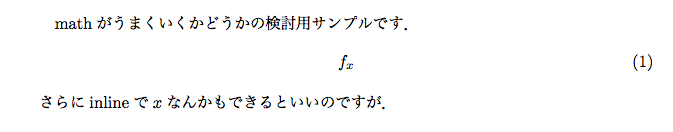
\includegraphics[width=6cm]{./Math.png}
\caption{}
\label{default}\end{center}\end{figure}
\subsubsection{【コード解説】}
\paragraph{evaluate\_plugin\_block}
すこしトリッキーだったので,メモです.
\begin{lstlisting}[style=customRuby]
  def evaluate_plugin_block(str, buf = nil)
    buf ||= @output.container
    str.split(/(\0\d+\0)/).each do |s|
      if s[0, 1] == "\0" and s[-1, 1] == "\0"
        buf << @output.inline_plugin(plugin_block(s[1..-2].to_i))
      else
        buf << @output.text(s)
      end
    end
    buf
  end
\end{lstlisting}
としてinline\_pluginはblock\_pluginと違った扱いになっています.bufに一度溜め込んでそれを@fに吐いているようです.
そこで,@output.inline\_pluginで行き着く先が,LatexOutputの
\begin{lstlisting}[style=customRuby]
  def inline_plugin(src)
    tmp=[]
    if ( /(\w+)\((.+)\)/ =~ src ) or ( /(\w+).\'(.+)\'/ =~src ) or (/(\w+)/ =~ src)
      tmp = [$1,$2]
    end

    case tmp[0]
    when 'dmath'
      "\\begin{equation}\n#{tmp[1]}\n\\end{equation}"
    when 'math'
      "\$#{tmp[1]}\$"
    else
      %Q(<span class="plugin">{{#{src}}}</span>)
    end
  end
\end{lstlisting}
としてmath,dmathを処理しています.必要ならそれ以外のinlineもここに付け足すことで対応できます.

\paragraph{snake\_nameがlatexで引っかかる}
math環境の移し替えはうまくいったが,underscore\_namesがすべて引っかかるequationとして引っかかる.
\begin{quote}\begin{verbatim}
\usepackage{underscore}
\end{verbatim}\end{quote}
だけでもできるようだが,できればto\_latexで対応したい.ということで,paragraphにescape\_snake\_namesを入れた.

paragraphはpreformattedからは呼ばれない.しかし,\verb|$$|や\verb|\begin{equation}...\end{equation}|が含まれる.そこで
一旦全置換してそこだけ戻すようにした.gsubのなかでなんどもできるか自信がなくて.二重のgsubにしているが...
\begin{lstlisting}[style=customRuby]
  def escape_snake_names(str)
    str.gsub!(/_/,"\\_")
    str.gsub!(/\$.+?\$/){ |text| text.gsub!(/\\_/,"_")  }
    str.gsub!(/equation.+?equation/m){ |text| text.gsub!(/\\_/,"_") }
  end

  def paragraph(lines)
    lines.each{|line| line = escape_snake_names(line) }
    @f << "#{lines.join("\n")}\n\n"
  end
\end{lstlisting}
gsub!で置換できなかったときには,nilが返るので対応.なんかえらく冗長.
\begin{lstlisting}[style=customRuby]
  def escape_snake_names(str)
    str.gsub!(/_/,"\\_")
    str.gsub!(/\$.+?\$/){ |text|
      if text =~ /\\_/ then
        text.gsub!(/\\_/,"_")
        else
        text
      end
    }
    str.gsub!(/equation.+?equation/m){ |text|
      if text =~ /\\_/ then
        text.gsub!(/\\_/,"_")
        else
        text
      end
    }
    str
  end
\end{lstlisting}
\paragraph{escape\_snake\_namesを改良(2016/02/14)}
gemへの公開にあたって冗長部を簡略化.verbだけはここを切り出した検証とは違う.testにuriを埋め込んでverb変換とsnakeを検証.
\begin{lstlisting}[style=customRuby]
  def escape_snake_names(str)
    str.gsub!(/_/,"\\_")
    patterns = [/\$(.+?)\$/ , /\\verb\|(.+?)\|/, /equation(.+?)equation/m ]
    patterns.each{|pattern|
      str.gsub!(/\\_/,"_")    if str.match(pattern)
    }
    str
  end
\end{lstlisting}
\paragraph{escape\_snake\_namesを再改良(2016/02/16)}
underscoreではincludeなどでsnake\_named\_fileも変換してしまい,だめ.hiki2latexで対応.

上のやり方では,うまくいかない場合が存在.元へ戻す.
\begin{lstlisting}[style=customRuby]
def escape_snake_names(str)
    str.gsub!(/_/,"\\_")
    patterns = [/\$(.+?)\$/ , /\\verb\|(.+?)\|/, /equation(.+?)equation/m ]
    patterns.each{|pattern|
#      str.gsub!(/\\_/,"_")    if str.match(pattern)                                                                                   
      str.gsub!(pattern){|text|
        if text =~ /\\_/ then
          text.gsub!(/\\_/,'_')
        else
          text
        end
      }
    }
    str
  end
\end{lstlisting}
さらに
tableでescape\_snake\_namesを通ってなかった.
\begin{quote}\begin{verbatim}
#        buf << "#{ele} &"
       buf << escape_snake_names(ele)+" &"
\end{verbatim}\end{quote}
\subsubsection{【copyright】}
cc by Shigeto R. Nishitani, 2015


\pagebreak
\subsection{table環境}

\subsubsection{【概要】}
hiki2latexのtable処理部

\subsubsection{【仕様】}\begin{itemize}
\item hiki記法の表をtabularへ変換
\item 連結作用素に対応
\item 行連結では中心に表示を移動
\item 縦罫は基本使わない
\item 横罫はheader内枠と上下外枠のみ
\end{itemize}
\subsubsection{【hiki】}\begin{quote}\begin{verbatim}
||>A11||>A12||
||^^A21||A22||>A23||
||A11||^A22||A12||
||A21||A23||
\end{verbatim}\end{quote}
\begin{table}[htbp]\begin{center}
\caption{}
\begin{tabular}{lllll}
\hline
\multicolumn{2}{l}{A11 }  &\multicolumn{2}{l}{A12 }  \\ \hline
 &A22  &\multicolumn{2}{l}{A23 }  \\
A21  &A11  &A22  &A12  \\
 &A21  & &A23  \\
\hline
\end{tabular}
\label{default}
\end{center}\end{table}
%for inserting separate lines, use \hline, \cline{2-3} etc.

\subsubsection{【latex】}\begin{lstlisting}[style=]
¥begin{center}¥begin{table}[htbp]¥begin{tabular}{ccccc}
¥hline
¥multicolumn{2}{c}{A11 }  &¥multicolumn{2}{c}{A12 }  &  ¥¥ ¥hline
 &A22  &¥multicolumn{2}{c}{A23 }  &  ¥¥
A21  &A11  &A22  &A12  &  ¥¥
 &A21  & &A23  &  ¥¥
¥hline
¥end{tabular}¥end{table}¥end{center}
%横罫を入れる場合は, ¥hline, ¥cline{2-3}などで.
\end{lstlisting}
\begin{figure}[htbp]\begin{center}
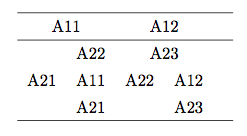
\includegraphics[width=6cm]{./table.png}
\caption{}
\label{default}\end{center}\end{figure}
\subsubsection{【コード解説】}
元のHTMLOutputではそれぞれの要素で対応していたが,LatexOutputではtable\_closeにて
\begin{lstlisting}[style=customRuby]
    def table_close
      @f << make_table
    end
\end{lstlisting}
としている.make\_tableは下請けにmake\_matrixを読んでおり,ここでほぼ全ての作業をしている.作業内容は
\begin{itemize}
\item matrixを作る
\item 縦連結を処理\begin{itemize}
\item 縦連結の数(rs)だけ下行に追加
\item 連結の中心(c\_rs)に内容を表記
\end{itemize}
\item 横連結をmulticolumnで処理\begin{itemize}
\item ついでに最大列数(max\_col)を記録
\end{itemize}
\end{itemize}\begin{lstlisting}[style=customRuby]
bob% cat table.rb
cont = File.readlines("table")

cont.each{|line|
  p tmp=line.split('||')
}

t_matrix=[]
cont.each{|line|
  tmp=line.split('||')
  tmp.slice!(0)
  tmp.slice!(-1) if tmp.slice(-1)=="\n"
  tmp.each_with_index{|ele,i| tmp[i] = ele.match(/\s*(.+)/)[1]}
  t_matrix << tmp
}

t_matrix.each_with_index{|line,i|
  line.each_with_index{|ele,j|
    if ele=~/\^+/ then
      t_matrix[i][j]=""
      rs=$&.size
      c_rs=rs/2
      rs.times{|k| t_matrix[i+k+1].insert(j,"")}
      t_matrix[i+c_rs][j]=$'
    end
  }
}
p t_matrix

max_col=0
t_matrix.each_with_index{|line,i|
  n_col=line.size
  line.each_with_index{|ele,j|
    if ele=~/>+/ then
      cs=$&.size
      t_matrix[i][j]= "\\multicolumn{#{cs+1}}{c}{#{$'}} "
      n_col+=cs
    end
  }
  max_col = n_col if n_col>max_col
}
p t_matrix
p max_col
\end{lstlisting}

\pagebreak
\subsection{source code環境}
\subsubsection{【概要】}
latexのlistingsスタイルを使って,source codeの色付き表示が可能に.

\subsubsection{【hiki2latexの変更】}
hikidoc2texで使われているのを参照して,
\begin{lstlisting}[style=customRuby]
  def block_preformatted(str, info)
    if (@listings==true and info!=nil) then
      style='customRuby' if info=='ruby'
      style='customCsh' if (info=='tcsh' or info=='csh')
      style='customTeX' if info=='tex'
      style='customJava' if info=='java'
      preformatted_with_style(str,style)
    else
      preformatted(text(str))
    end
  end

  def preformatted(str)
    @f.slice!(-1)
    @f << "\\begin{quote}\\begin{verbatim}\n"
    @f << str+"\n"
    @f << "\\end{verbatim}\\end{quote}\n"
  end

  def preformatted_with_style(str,style)
    @f.slice!(-1)
    @f << "\\begin{lstlisting}[style=#{style}]\n"
    @f << str+"\n"
    @f << "\\end{lstlisting}\n"
  end
\end{lstlisting}
opt周りは,
\begin{lstlisting}[style=customRuby]
        opt.on('--listings', 'use listings.sty for preformat with style.') {@listings=true }
\end{lstlisting}
としている.これをHikiDocへ渡す時は,
\begin{lstlisting}[style=customRuby]
    def plain_doc(file)
      if @listings==true then
        puts listings_preamble
      elsif @pre==nil then
        puts "\\documentclass[12pt,a4paper]{jsarticle}"
        puts "\\usepackage[dvipdfmx]{graphicx}"
      else
        puts File.read(@pre)
      end
      puts "\\begin{document}"
      puts File.read(@head) if @head!=nil
      puts HikiDoc.to_latex(File.read(file),{:listings=>@listings})
      puts File.read(@post) if @post!=nil
      puts "\\end{document}"
    end
\end{lstlisting}
後ろのoptions={}の中にhashで登録している.texのstyleはlisting\_preambleで打ち出すようにしている.

listingsの設定は以下の通り.
\begin{lstlisting}[style=customTeX]
\documentclass[10pt,a4paper]{jsarticle}
\usepackage[dvipdfmx]{graphicx}
\usepackage[dvipdfmx]{color}
\usepackage{listings}
% to use japanese correctly, install jlistings.
\lstset{
  basicstyle={\small\ttfamily},
  identifierstyle={\small},
  commentstyle={\small\itshape\color{red}},
  keywordstyle={\small\bfseries\color{cyan}},
  ndkeywordstyle={\small},
  stringstyle={\small\color{blue}},
  frame={tb},
  breaklines=true,
  numbers=left,
  numberstyle={\scriptsize},
  stepnumber=1,
  numbersep=1zw,
  xrightmargin=0zw,
  xleftmargin=3zw,
  lineskip=-0.5ex
}
\lstdefinestyle{customCsh}{
  language={csh},
  numbers=none,
}
\lstdefinestyle{customRuby}{
  language={ruby},
  numbers=left,
}
\lstdefinestyle{customTex}{
  language={tex},
  numbers=none,
}
\lstdefinestyle{customJava}{
  language={java},
  numbers=left,
}
\end{lstlisting}\begin{quote}\begin{verbatim}
\begin{lstlisting}[style=customRuby]
  def block_preformatted(str, info)
    if (@listings==true and info!=nil) then
      style='customRuby' if info=='ruby'
      style='customCsh' if (info=='tcsh' or info=='csh')
      style='customTeX' if info=='tex'
...
\end{lstlisting}
\end{verbatim}\end{quote}

\pagebreak
\end{document}
